%----------------------------------------------------------------------------------------
%       CHAPTER 7
%----------------------------------------------------------------------------------------

\cleardoublepage

\chapterimage{chx-biogeo.png} % Chapter heading image

\chapter{Ocean biogeochemical cycles}\label{ch:ocean-biogeochem}

\hfill \break

\vspace{24mm}

\noindent

%------------------------------------------------
\newpage
%------------------------------------------------

\section*{READ.ME}

You will need the following \textit{re-starts} files prior to embarking on the experiments in the Chapter.
\vspace{1mm}

\begin{itemize}[noitemsep]
\vspace{2mm}
\item [7.1] This is the basic single (\(PO_{4}\)) nutrient biological export scheme configuration.
\vspace{-1mm}\small\begin{verbatim}
$ wget --no-check-certificate http://www.seao2.info/cgenie_output/ ...
muffin.CB.p_worbe2.BASES.ridgwelletal.SPIN.tar.gz
\end{verbatim}\normalsize\vspace{-1mm}
\vspace{2mm}
\item [7.2] A single (\(PO_{4}\)) nutrient biological export scheme but in a higher (vertical) resolution ocean.
\vspace{-1mm}\small\begin{verbatim}
$ wget --no-check-certificate http://www.seao2.info/cgenie_output/ ...
muffin.CB.p_worjh2.BASES.caoetal.SPIN.tar.gz
\end{verbatim}\normalsize\vspace{-1mm}
World Ocean\ Atlas modern (\(PO_{4}\)) climatology (re-gridded/interpolated observations), re-gridded to the same ocean grid as \textsf{\footnotesize EXAMPLE.worjh2.Caoetal2009.SPIN}
\vspace{-1mm}\small\begin{verbatim}
$ wget --no-check-certificate http://www.seao2.info/cgenie_output/ ...
worjh2.p_an.200709.nc
\end{verbatim}\normalsize\vspace{-1mm}
World Ocean\ Atlas modern (\(O_{2}\)) climatology (re-gridded/interpolated observations), re-gridded to the same ocean grid as \textsf{\footnotesize EXAMPLE.worjh2.Caoetal2009.SPIN}
\vspace{-1mm}\small\begin{verbatim}
$ wget --no-check-certificate http://www.seao2.info/cgenie_output/ ...
worjh2.o_an.200709.nc
\end{verbatim}\normalsize\vspace{-1mm}
\vspace{2mm}
\item [7.3] 
\small \begin{verbatim}
$ wget --no-check-certificate http://www.seao2.info/cgenie_output/ ...
muffin.CB.p_worjh2.BASES.crichtonetal.STND.SPIN.tar.gz
$ wget --no-check-certificate http://www.seao2.info/cgenie_output/ ...
muffin.CB.p_worjh2.BASES.crichtonetal.TDEP.SPIN.tar.gz
\end{verbatim} \normalsize
\vspace{2mm}
\item [7.4] 
\small\begin{verbatim}
$ wget --no-check-certificate http://www.seao2.info/cgenie_output/ ...
muffin.CB.p_worjh2.BASESFe.FeMIP.SPIN.tar.gz
\end{verbatim}\normalsize
\vspace{2mm}
\item [7.5] 
(as per for 7.4)
\end{itemize}

\vspace{2mm}
\noindent Extract the results in the usual way and in the usual place ... and return to \textsf{\footnotesize genie-main} in the usual way ... all ... as usual.

%------------------------------------------------
\newpage
%------------------------------------------------

\section*{The ocean's biological pump}

In this Chapter we'll step through some of the facets of the cycle of carbon (and nutrients) in the ocean -- the 'biological pump'. And then in a later section we'll look at the same processes but in a different way -- through the lens of 'geoengineering', and hopefully learn something further about how everything 'works' regardless of the desirability and or effectiveness, or not, of geoengineering.

\textbf{muffin} incorporates a variety of options for simulating biological export production. To date, these have all been rooted in what is effectively a nutrient mass balance approach to estimating export production, nicely encapsulated by Ernst Maier-Reimer as: “\textit{conceptually not a model of biology in the ocean but rather a model of biogenically induced chemical fluxes [from the surface ocean]}” [\textit{Maier-Reimer,} 1993]. Hence in schemes of this nature -- which we will term ‘biogenic  flux’ schemes --  there is no attempt to explicitly account for changes in cell numbers/biomass and hence, nor zooplankton, which will impact a bias particularly in the seasonal time-dependent response of export. Previous biogenic flux schemes utilized in  \textbf{muffin}  considered a single nutrient (P limitation) only and took either restoring to observations [Cameron et al., 2005] or explicit P-limitation [Ridgwell et al., 2007a,b] approaches. More recently, additional limitation by iron (P+Fe) has been implemented, while nitrogen cycling (including N fixation and denitrification) and hence P+N limitation, has been implemented and explored in the context of extreme nutrient and oxygen cycle perturbation associated with the Cretaceous Oceanic Anoxic Events [Monteiro et al., 2012; Naafs et al., 2029]. Work currently in development includes the additional consideration of Si limitation (P+Si limitation) control on production of diatoms vs. non-diatoms following \textit{Ridgwell et al.} [2002].

Overall, biological production and net export of particulate (POM) and dissolved (DOM) organic matter plus calcium carbonate (\(CaCO_{3}\)) are directly determined by the availability of nutrients (phosphate and/or total dissolved iron and/or \(NO^{2-}_{3}\) (and/or \(NH^{+}_{4}\)) and/or dissolved silica) together with the degree to which physical conditions, particularly light and temperature, are conducive to growth. DOM is remineralzied (transformed back to inorganic dissolved constituents) relatively rapidly (a ca. annual time-scale) and hence mostly at or close to the ocean surface, while POM is assumed to sink down into the ocean interior. See: \textit{Hülse at al.} [2017]\footnote{Hülse, D., S. Arndt, J.D. Wilson, G. Munhoven, and A. Ridgwell, Understanding the causes and consequences of past marine carbon cycling variability through models, Earth-Science Reviews 171, dx.doi.org/10.1016/j.earscirev.2017.06.004 (2017).} for a comprehensive review (esp. of implementation in models).

Note that a full description of the various biological and ocean interior remineralization schemes (together constituting the biological pump) is not given here as background. Rather, the relevant provided references should be read (rather than e.g. downloaded and immediately forgotten ...).

%------------------------------------------------
\vspace{1mm}
\noindent\rule{4cm}{0.5pt}
\vspace{2mm}
%------------------------------------------------

%------------------------------------------------
\newpage
%------------------------------------------------

\noindent What should you be thinking of looking at in terms of model output to understanding something about the role of the oceans biological pump in the Earth system (and climate dynamics)? Each subsequent exercise will direct you to some of the outputs to analyze/visualize that are directly relevant to the question (model experiment). In addition to that, what follows is a brief general over-view of relevant fields.

\begin{itemize}[noitemsep]

\vspace{2mm}
\item Firstly, it is worth noting, if you have not already, the summary text file: 
\\\textsf{\footnotesize biogem\_year\_yyyy\_yyy\_diag\_GLOBAL\_AVERAGE.res}
where \textsf{\footnotesize yyyy\_yyy} is the mid-point of the annual average year saved. Hence for the provided 10,000 year spin-up \\\textsf{\footnotesize muffin.CB.p\_worbe2.BASES.ridgwelletal.SPIN}, the file is: \\\textsf{\footnotesize biogem\_year\_09999\_500\_diag\_GLOBAL\_AVERAGE.res}. 

\vspace{1mm}
Each of these files contains summary information associated with each \textit{time-slice}. Model properties that you might pay particular attention to includes:

\vspace{1mm}
\begin{itemize}[noitemsep]
\item
\vspace{1mm}
\vspace{-0mm}\footnotesize\begin{verbatim}
 ATMOSPHERIC PROPERTIES
 Atmospheric pCO2             :    278.000 uatm
 Atmospheric pCO2_13C         :     -6.500 o/oo
\end{verbatim}\normalsize\vspace{1mm}
is a useful place to find e.g. the final (annual average) value of atmospheric \(pCO_{2}\) (rather than searching to the end of the relevant \textit{time-series} file).
\item
\vspace{1mm}
\vspace{-0mm}\footnotesize\begin{verbatim}
 BULK OCEAN PROPERTIES
 Ocean DIC              ..... :   2211.435 umol kg-1 <->   0.2977295E+19 mol
\end{verbatim}\normalsize\vspace{1mm}
reflecting how much carbon is stored in the ocean, 
\vspace{0mm}\footnotesize\begin{verbatim}
 Ocean PO4              ..... :      2.154 umol kg-1 <->   0.2899897E+16 mol
\end{verbatim}\normalsize\vspace{0mm}
the ocean nutrient (here: phosphorous) inventory,
\vspace{-0mm}\footnotesize\begin{verbatim}
 Ocean O2               ..... :    221.288 umol kg-1 <->   0.2979245E+18 mol
\end{verbatim}\normalsize\vspace{0mm}
is the average concentration of dissolved oxygen in the ocean (and its inventory).
\item
\vspace{1mm}
\vspace{-0mm}\footnotesize\begin{verbatim}
 SURFACE EXPORT PRODUCTION
 Export flux POC              :    204.253 umol cm-2 yr-1 <->   0.7505843E+15 mol yr-1
 Export flux CaCO3            :     28.624 umol cm-2 yr-1 <->   0.1051875E+15 mol yr-1
\end{verbatim}\normalsize\vspace{1mm}
fluxes reflecting the global biological export of particulate organic matter and calcium carbonate, and then
\vspace{-0mm}\footnotesize\begin{verbatim}
 SURFACE EXPORT PRODUCTION
 Export flux POC              :    204.253 umol cm-2 yr-1 <->   0.7505843E+15 mol yr-1
 Export flux CaCO3            :     28.624 umol cm-2 yr-1 <->   0.1051875E+15 mol yr-1
\end{verbatim}\normalsize\vspace{0mm}
is the residual flux that actually reaches the sea-floor.
\end{itemize}

\vspace{1mm}
Finally, there is a summary of the summary, which is often the most useful of all:
\vspace{1mm}
\begin{itemize}[noitemsep]
\item
\vspace{-0mm}\footnotesize\begin{verbatim}
 SURFACE EXPORT & SEDIMENT DEPOSITION (RAIN) FLUX SUMMARY
 Total POC export   :   0.7505843E+15 mol yr-1 =   9.007 PgC yr-1
 Total CaCO3 export :   0.1051875E+15 mol yr-1 =   1.262 PgC yr-1
 Total POC rain     :   0.8654062E+14 mol yr-1 =   1.039 PgC yr-1
 Total CaCO3 rain   :   0.5191799E+14 mol yr-1 =   0.623 PgC yr-1
\end{verbatim}\normalsize\vspace{0mm}
where carbon fluxes are also given in helpful and literature-friendly units of \(PgCyr^{-1}\).
\end{itemize}

%------------------------------------------------
\newpage
%------------------------------------------------
%
\vspace{2mm}
\item Secondly, there are \textit{time-series} files related to much of the above \textit{time-slice} summary information, e.g.: 

\vspace{1mm}
\begin{itemize}[noitemsep]
\item []
\begin{itemize}[noitemsep]
\item [] \textsf{\footnotesize biogem\_series\_fexport\_POC.res}
\item [] \textsf{\footnotesize biogem\_series\_fexport\_POP.res}
\item [] \textsf{\footnotesize biogem\_series\_fexport\_CaCO3.res}
\end{itemize}
\vspace{1mm}
are the \textit{time-series} of the carbon and phosphorous of particulate organic matter export, and that for \(CaCO_{3}\), and
\vspace{1mm}
\begin{itemize}[noitemsep]
\item [] \textsf{\footnotesize biogem\_series\_ocnsed\_POC.res}
\item [] \textsf{\footnotesize biogem\_series\_ocnsed\_POP.res}
\item [] \textsf{\footnotesize biogem\_series\_ocnsed\_CaCO3.res}
\end{itemize}
\vspace{1mm}
the corresponding fluxes at the sea-floor.
\begin{itemize}[noitemsep]
\item [] \textsf{\footnotesize biogem\_series\_ocn\_PO4.res}
\end{itemize}
will tell you how what the global annual average nutrient concentration is (left) at the surface, and
\begin{itemize}[noitemsep]
\item [] \textsf{\footnotesize biogem\_series\_ocn\_O2.res}
\end{itemize}
the average concentration dissolved oxygen in the ocean and at the sea-floor.
\end{itemize}

\vspace{2mm}
\item Thirdly, as always -- \textbf{netCDF} outputs.

\begin{itemize}[noitemsep]
\vspace{1mm}
\item In the 2D \textbf{netCDF}:
\vspace{1mm}
\begin{itemize}[noitemsep]
\item [] \textsf{\footnotesize bio\_export\_POC}
\item [] \textsf{\footnotesize bio\_export\_POP}
\item [] \textsf{\footnotesize bio\_export\_CaCO3}
\end{itemize}
== spatial fields of the export flux of \(POC\), \(POP\), \(CaCO_{3}\), and variables with \textsf{\footnotesize focnsed} in place of \textsf{\footnotesize bio\_export} in its name the flux distributions to the sea-floor.

\vspace{1mm}
Derived from these:
\vspace{1mm}
\begin{itemize}[noitemsep]
\item [] \textsf{\footnotesize misc\_sur\_rCaCO3toPOC}
\item [] \textsf{\footnotesize misc\_sur\_rPOCtoPOP}
\end{itemize}
are the rations of \(CaCO_{3}/POC\) and \(POC/POP\), respectively.
\vspace{1mm}
\\There are then some fields for surface and benthic tracer concentrations, such as of phosphate.
\vspace{1mm}
\item In the 3D \textbf{netCDF}, \textsf{\footnotesize bio\_*} are the 3D spatial distributions of particles setting down through the ater column -- \textsf{\footnotesize bio\_fpart\_*} is the particulate flux density, \textsf{\footnotesize bio\_fparttot\_*} the total flux associated with each grid point, and \textsf{\footnotesize bio\_fpartnorm\_*} are the fluxes in the water column normalized to the export flux out of the base of the surface ocean layer.
\vspace{1mm}
\\Also see spatial distributions of dissolved carbon, nutrients, and oxygen etc.
\end{itemize} 

\end{itemize}

%------------------------------------------------
\vspace{1mm}
\noindent\rule{4cm}{0.5pt}
\vspace{2mm}
%------------------------------------------------

\noindent From just the \textit{spin-up} experiment results you can explore and/or plot some of these fields.

%------------------------------------------------
\newpage
%------------------------------------------------

\section{Basic controls on biological productivity}

The following exercises  will utilize one of the more basic representations of the biological pump -- one with only a single nutrient (PO$_{4}$) potentially limiting to biological export, considered. The scheme is described in full in \textit{Ridgwell et al.} [2007]\footnote{Ridgwell, A., et al., Marine geochemical data assimilation in an efficient Earth System Model of global biogeochemical cycling, Biogeosci. 4, 87-104 (2007). }. Note that this specific configuration of the (modern) ocean model accounts only for 8 layers in the ocean (but spanning the same \(0-5000 \) water depth range as the 16-level model configuration used in evaluating AMOC stability as wel as fossil fuel \(CO_{2}\) uptake). Although the limited vertical resolution of the 8-level model places additional constraints on the ability of the model to reproduce features such as oxygen minimum zones in the ocean, it does enable a much shorter run-time (via a longer time-step in the model as well as about a \(50\%\) reduction in the total number of ocean cells). Hence we are making  trade-off between model fidelity (in reproducing observed distribution of tracers in the modern ocean) and speed (and hence the ability to more effectively 'play' with the Earth system in a relatively short amount of real time).

\vspace{1mm}

We will consider the following scientific questions as a starting point, and then devise some model experiments to address them them all:

\begin{enumerate}[noitemsep]
\vspace{1mm}
\item What would the Earth look like with no biological production in the ocean? Specifically: how important is the biological pump in controlling atmospheric \(pCO_{2}\) and how much higher would \(pCO_{2}\) be in the absence of biology (and a biological pump) in the ocean?
\vspace{1mm}
\item Conversely, is the biological pump operating at its maximum efficient in the ocean today, and if not, how much more could atmospheric \(pCO_{2}\) conceivably be lowered by increasing its strength/efficiency?
\vspace{1mm}
\item Associated with \#1 and \#2 -- how does the biological pump affect the distribution and hence availability of dissolved oxygen in the ocean? (How more oxygenated would the ocean be with no export of organic matter into the ocean interior, and how much more severe would oxygen depletion be if plankton were able to utilize all the nutrients at the ocean surface?)
\vspace{1mm}
\item If carbon and nutrients are returned back to solution (remineralized) much closer to the ocean surface, does atmospheric \(pCO_{2}\) increase or decrease??? (The faster return of DIC to the ocean surface will tend to increase \(pCO_{2}\) while the return of nutrients will tend to enhance biological productivity and decrease \(pCO_{2}\) ... so the answer is not necessarily intuitive and hence why we build and run computer models.)
\vspace{1mm}
\item What about if carbon and nutrients are much more efficiently exported into the very deepest parts of the ocean -- does \(pCO_{2}\) increase or decrease (and what happens to e.g. \([O_{2}]\))?
\vspace{1mm}
\item What is the role of the calcium carbonate (\(CaCO_{3}\)) 'counter pump'? How much higher is \(pCO_{2}\) in the presence of calcifying organisms in the ocean compared to just organic matter production and cycling?
\vspace{1mm}
\item What is the role of large-scale ocean circulation in dictating the cycling of carbon and nutrients and hence setting the patterns of ocean oxygenation. (For example, how would a chance in the AMOC impact atmospheric \(pCO_{2}\)?)
\vspace{1mm}
\item What about feedbacks with climate -- how does changing global surface temperature (and hence ocean circulation patterns and sea-ice extent) modulate the impact of changes to the biological pump in the ocean? Is the resulting feedback positive or negative (and why)?
\end{enumerate}
\vspace{1mm}

%------------------------------------------------
\newpage
%------------------------------------------------
%
The associated experiments would ideally be run for several thousand and maybe as long as 5000 years in order to obtain a complete new (quasi) steady state of carbon and nutrient cycling in the ocean. However, the main impacts in the ocean and on atmospheric \(pCO_{2}\) tend develop relatively rapidly (decades). Hence model experiments could be run for a few 10s or perhaps a few 100 years to see something 'happen'.  A full 5000 years can also be run but periodically downloading and viewing the results as the experiment progresses and not necessarily waiting until the end of the experiment, or even ever looking at the final state! As always -- if possible -- run a representative (or perhaps the most extreme, such as shutting off the biological pump entirely) experiment for 5,000 or even 10,000 years, and answer for yourself how long the different facets of the system (ocean circulation if that has been modified or if there is a feedback with climate, total global export production, mean ocean \([O_{2}]\)) take to adjust.

%------------------------------------------------
\vspace{1mm}
\noindent\rule{4cm}{0.5pt}
\vspace{2mm}
%------------------------------------------------

\noindent All the experiments in this first subsection will start from the same \textit{re-start}\footnote{As per described in Ridgwell et al. [2007].} and are based on the same \textit{user-config}\footnote{The same \textit{user-config} as used to generate the \textit{re-start} (with the exception that the atmospheric \(CO_{2}\) concentration is no longer prescribed).}. To run an e.g. 100 year experiment (but it need not be this -- see above) using the template \textit{user-config} and provided \textit{re-start} would look like:
\vspace{-1mm}\small\begin{verbatim}
./runmuffin.sh muffin.CB.p_worbe2.BASES LABS ch07.1.8lvl.EXPT 
   100 muffin.CB.p_worbe2.BASES.ridgwelletal.SPIN
\end{verbatim}\normalsize\vspace{-1mm}
(When you run new experiments, remember to copy and rename the provided \textit{user-config} \textsf{\footnotesize ch07.1.8lvl.EXPT} in order to create new and unique experiments each time.)

\vspace{1mm}

Whatever you plan to do re. perturbation experiments to explore the working of the ocean's biological pump, the first thing to do, is to run a \textbf{control experiment} for however long you have decided to run all the actual experiment experiments for. (You need not wait for this to finish, but can submit it as a \textit{job} to the cluster and get on with running some real experiment experiments.) The control experiment can simply be derived (copied) from \textsf{\footnotesize ch07.1.8lvl.EXPT}, with no further alterations in parameter values needed. In this \textit{user-config}, the value of atmospheric  \(pCO_{2}\) is not prescribed (there is no \textit{forcing} defined) and hence \(pCO_{2}\) is free to respond to any change in parameters. In the case of the control -- there are no changes in the biological pump parameters compared to the \textit{spin-up}, so you should see no (or little) drift in \(pCO_{2}\) occurring. 
A substantive drift in the control experiment (e.g. \(10s\) of \(ppm\) of \(CO_{2}\) in the atmosphere over 100 years) is your way of knowing that you have either used the wrong \textit{re-start} or have accidently modified key parameters in your control experiment \textit{user-config} compared to those used to generate the \textit{re-start}.

\vspace{1mm}
Plan in advance  the output you want to view and make sure it is going to appear(!) In the \textit{user-config} -- check that the results/output select 'level' is going to give you the output you are expecting. In the example \textit{user-config}, this is specified by:
\vspace{-1mm}\small\begin{verbatim}
bg_par_data_save_level=7
\end{verbatim}\normalsize\vspace{-1mm}
(Refer to Section 14.4 and Appendix I, for more details on how different (2D and 3D) \textit{time-slice} variable fields and \textit{time-series} are selected to be included in the model output.)

\vspace{1mm}
Also note that in the example \textit{user-config} provided, netCDF time-slices are only saved at the very end (final annual average) of the model experiment, regardless of how long that is:
\vspace{-1mm}\small\begin{verbatim}
bg_par_infile_slice_name='save_timeslice_NONE.dat'
\end{verbatim}\normalsize\vspace{-1mm}
You may want to request more frequent saving of the spatial fields -- see Section 15.2 (nd 15.3).

%------------------------------------------------
\newpage
%------------------------------------------------
%
\noindent In terms of the specific 'questions' at the start (the numbering system is the same in the following), the parameters and parameter values to change and well as what to 'look for' are:
\vspace{1mm}

\begin{enumerate}[noitemsep]

\vspace{1mm}
\item The parameter scaling the rate of nutrient uptake (and hence biological export) is:
\vspace{-1mm}\small\begin{verbatim}
# maximum rate of conversion of dissolved PO4 into 
# organic matter by phytoplankton (mol kg-1 yr-1)
bg_par_bio_k0_PO4=1.9582242E-06
\end{verbatim}\normalsize\vspace{-1mm}
(in units of \(mol\:PO_{4} \:kg^{-1} \:yr^{-1}\)). Setting this to zero would 'turn off' completely the biological pump, leaving you with a abiotic ocean.
\vspace{1mm}
\\What to look for? The value of atmospheric \(pCO_{2}\). You might also confirm that biological export really is zero (so check the fluxes).
\vspace{1mm}
\\To obtain these values you can refer to the respective time-series results files. Or,  the summary text file: \textsf{\footnotesize biogem\_year\_yyyy\_yyy\_diag\_GLOBAL\_AVERAGE.res}
where \textsf{\footnotesize yyyy\_yyy} is the mid-point of the annual average year saved. Each of these files contains summary information associated with  each \textit{time-slice}, including mean atmospheric composition, mean ocean composition, biological export fluxes. The same information can be found in various \textit{time-series} files, but sometimes it is simply easier to find it here in one place!

\vspace{1mm}
\item Similar to above -- nutrient uptake and the strength of the biological pump can be enhanced by increasing the value of the parameter \texttt{bg\_par\_bio\_k0\_PO4} (maybe 10 times larger?).
The question is then what does the ocean and atmospheric \(pCO_{2}\) look like if the biological pump is operating at its maximum rate and (almost) all nutrients are consumed at the surface. (If you find that there are regions of nutrients that never get fully consumed ... why?)

\vspace{1mm}
\item For the question on dissolved oxygen (\([O_{2}]\)) availability in the ocean interior -- the parameters and experiments are as above, except you are looking for how the mean and distribution of dissolved oxygen in the ocean changes. Mean ocean [\(O_{2}\)] values can be obtained form time-series of the summary file. Spatial distributions are recorded in the \textit{netCDF} output. You might view horizontal or vertical slices (from 3D), or benthic distributions (2D). Think about where animals tend to live and where they could potentially be impacted if export from the ocean surface was much higher than 'today' (the \textit{spin-up}).

\vspace{1mm}
\item The parameter controlling the depth-scale (and vertical distribution) at which particulate organic matter (POM) is remineralizated in the ocean interior is controlled by:
\vspace{-1pt}\small\begin{verbatim}
bg_par_bio_remin_POC_eL1=550.5195
\end{verbatim}\normalsize\vspace{-1pt}
(units of \(m\)). Reducing the value of this parameter forces a greater proportion of sinking POM to be remineralized closer to the surface, while a larger value pushes particulate organic matter  (and associated carbon and nutrients) deeper down on average into the ocean interior.

%
\noindent What to look for? Largely as before -- the summary file is useful for atmospheric \(CO_{2}\), mean ocean {\(O_{2}\)}, and global (biological) export fluxes (as you might expect nutrients released closer to the ocean surface to result in greater surface ocean nutrient supply and hence fuel higher export). You might also consider the spatial patterns of nutrients and dissolved oxygen.
\\See \textit{Meyer et al.} [2016]\footnote{Meyer, K.M., A. Ridgwell, and J.L. Payne, The influence of the biological pump on ocean chemistry: implications for long-term trends in marine redox chemistry, the global carbon cycle, and the evolution of marine animal ecosystems, Geobiology, DOI: 10.1111/gbi.12176 (2016).} for an example of a study testing these sort of model changes and its implications (and hence ideas of what else to look for, and for 'reasonable' parameter values to test).

%------------------------------------------------
\newpage
%------------------------------------------------
%
\item Conversely, you can also increase the value of the depth scaling parameter in order to force a deeper mean depth of POM remineralization. You can also partition more of the total export into a POM form that is assumed to be resistent to degradation and is transported to the ocean floor completely unchanged (see: \textit{Ridgwell et al.} [2007]):
\vspace{-1pt}\small\begin{verbatim}
bg_par_bio_remin_POC_frac2=6.4591110E-02
\end{verbatim}\normalsize\vspace{-1pt}
Increasing this value forces a greater fraction of the POM exported from the surface ocean to reach the ocean floor.\footnote{See Ridgwell et al. 2007] for a description of how this all works.}

\vspace{1mm}
In both (4) and (5), it may not be obvious which way atmospheric \(pCO_{2}\) responds -- e.g. for (4) by returning nutrients more efficiently to the ocean surface, you increase export, and hence increase the fixation and removal of atmospheric \(CO_{2}\) from the ocean surface, drawing down atmospheric \(pCO_{2}\). BUT, at the same time, carbon released from \(POC\) (as \(DIC\)) through bacterial remineralization, also occurs at a shallower depth and is returned to the surface more efficiency ... tending to increase atmospheric \(pCO_{2}\) ... Just this problem -- 2 opposing effects with an uncertain net impact -- is exactly why (to find out the answer) you build and run numerical models of the system!

\vspace{1mm}
\item The export of \(CaCO_{3}\) from the ocean surface is calculated as a ratio to the export of \(POC\). By default, this ratio varies with the carbonate chemistry (saturation state) of the surface ocean, following \textit{Ridgwell et al.} [2007a] (and see also \textit{Ridgwell et al.} [2007b] and \textit{Ridgwell et al.} [2009]). 

\vspace{1mm}
The scaling parameter controlling the molar ratio of \(\frac{CaCO_{3}}{POC}\) is:
\vspace{-1pt}\small\begin{verbatim}
bg_par_bio_red_POC_CaCO3=0.044372
\end{verbatim}\normalsize\vspace{-1pt}
Setting this zero will effectively turn back the clock \(200Ma\) to a world prior to the evolution of planktic calcifiers (e.g. see: \textit{Ridgwell} [2005]), or conversely, a future world in which they are all driven extinction from ocean acidification ... 
\vspace{1mm}
\\What is the impact on atmospheric \(pCO_{2}\) of setting this to zero? From your knowledge of carbonate chemistry ... why does this happen? You might try e.g. doubling the value (and hence doubling the export of \(CaCO_{3}\) from the surface ocean). As well as \(pCO_{2}\), you might also look at fields of \(ALK\) (or other carbonate chemsitry parameters) in the ocean to see what other geochemical changes occur.

Because (rightly or wrongly) in the model, \(CaCO_{3}\) depends on surface ocean \(\Omega\) (w.r.t. calcite) you might explore what happens to \(CaCO_{3}\) production and export under a release of (fossil fuel) \(CO_{2}\) -- simplest here is to use the same re-start, and create and add a forcing to the \textit{user-config} to implement a large pulse or continuous \(CO_{2}\) flux to the atmosphere

%------------------------------------------------
\newpage
%------------------------------------------------
%
\item While it is possible to add a freshwater 'hosing' forcing (as used in an earlier Chapter/exercise) to modify large-scale ocean circulation, there is a simpler way just to 'turn off' the AMOC in the standard modern continental configuration of \textbf{muffin}.

\vspace{1mm}
The consequence of using the simplified \textbf{EMBM} atmosphere in conjunction with no topography over land, is that the net moisture transport from the Atlantic to the Pacific in the real world, is not reproduced. (This net transport is primarily a consequence of the blocking of Westerly transport moisture across the North American continent by e.g. the Rockies, while low latitude Trade Winds travel relatively topographically unrestricted through Central America, meaning that moisture transport from the Pacific to North Atlantic is partly blocked, while the reverse lower latitude transport is now.) To correct for this, there is a built-in prescribed moisture transport (technically, a negative salinity transport), principally from the North Atlantic to the North Pacific. In the model, there is a scaling parameter for the magnitude this transport ... which can be set to zero ... hence removing the prescribed moisture transport and likely leading to a collapse of the AMOC.

\vspace{1mm}
To kill (collapse) (hopefully) the \textbf{AMOC} in the modern continental configuration of \textbf{muffin}, set:

\vspace{-1mm}\small\begin{verbatim}
ea_28=0.0
\end{verbatim}\normalsize\vspace{-1mm}

Stuff to look for -- in addition to how the AMOC changes (e.g. plot the stream-function) how do the patterns of \([PO_{4}\)] and \([O_{2}\)], particularly in the deep North Atlantic change? What impact does this have on global export production, and ultimately on atmospheric \(pCO_{2}\)?

\vspace{1mm}
\item Finally, you might explore how in some (or all) of the above experiments,  a changing climate in response to changing atmospheric \(pCO_{2}\), in turn modulates the impacts through carbon-climate feedback. 

\vspace{1mm}
By default in the \textit{user-config}, climate-\(CO_{2}\) feedback is disabled:
\vspace{-1pt}\small\begin{verbatim}
ea_36=n
\end{verbatim}\normalsize\vspace{-1pt}
i.e. changing atmospheric \(pCO_{2}\) does not influence the climate system (which remains implicitly forced with a preindustrial radiative forcing value). This allows us to avoid complications arising due to carbon-climate feedback and hence obtain a the underlying response of the system to changing the biological pump in the ocean.

\vspace{1mm}
You can re-enable climate feedback by setting:
\vspace{-1mm}\small\begin{verbatim}
ea_36=y
\end{verbatim}\normalsize\vspace{-1mm}
Impacts may include (but not be limited to): ocean stratification (rapid warming) and/or changes in convection at high latitudes, increased/decreased sea-ice extent that affects the ocean surface area available for biological export, changing solubility of oxygen in sea-water.
\\Note that in this particular simple biological export scheme, there is no temperature-dependence of biological activity and hence export.

\end{enumerate}

%------------------------------------------------
\vspace{1mm}
\noindent\rule{4cm}{0.5pt}
\vspace{2mm}
%------------------------------------------------

\noindent And that pretty much wraps up all the main knobs that it is possible to play with using the very basic biological pump scheme in \textbf{muffin}. (However, a few further ideas follow ...)

%------------------------------------------------
\newpage
%------------------------------------------------

\subsection{Further ideas}

\noindent You might also play with the 'half saturtaion constant' for nutrient uptake (see \textit{Ridgwell et al.} [2007]):
\vspace{-2mm}\small\begin{verbatim}
#[PO4] M-M half-sat value (mol kg-1)
bg_par_bio_c0_PO4=2.1989611E-07
\end{verbatim}\normalsize\vspace{-1mm}
As set, this specifies that at a \(PO^{2-}_{4}\) concentration of about \(0.2 \mu mol \:kg^{-1} \), growth (net export) is restricted to half the maximum (and then declines further at even lower ambient nutrient concentration).

\vspace{1mm}
You might, for instance, try setting the value to zero, which assumes maximum growth can continue right up nutrient completely running out. This would be similar to assuming all the primary producers in the ocean had extremely small cell sizes (and hence low half saturation values) and were adapted to oligotrophic conditions.

Or, test an ocean dominated by assumed very large cell sizes and phytoplankton that struggle under anything other than fully eutrophic (high nutrient) conditions. e.g. you might try values of \(1.0 \mu mol \:kg^{-1}\) (\texttt{1.0E-06}) or even \(2.0 \mu mol \:kg^{-1}\) (\texttt{2.0E-06}) and see what happens, particularly to the pattern of surface nutrient concentrations and export.

%------------------------------------------------
\vspace{1mm}
\noindent\rule{4cm}{0.5pt}
\vspace{2mm}
%------------------------------------------------

\noindent By default, the update and export in organic matter, of carbon, occurs in a fixed 'Redfield' ratio, with \(PO^{2-}_{4}\). The classical value is \(106\) (i.e., for every mole of \(PO^{2-}_{4}\) taken up from the ocean, \(106\) moles of \(CO_{2}\) are removed (and fixed into organic matter). The parameter determining this is:
\vspace{-2mm}\small\begin{verbatim}
bg_par_bio_red_POP_POC=106.0
\end{verbatim}\normalsize\vspace{-2mm}
To change the default value (106.0), simply add a new line at the end of the \textit{user-config} file specifying the value you want. A larger number means that \(PO_{4}\) is being utilized more efficiently and more organic matter is being produced for the same nutrient consumption.

You should see impacts on atmospheric \(pCO_{2}\) and the oxygenation of the ocean interior form changing this.

%------------------------------------------------
\vspace{1mm}
\noindent\rule{4cm}{0.5pt}
\vspace{2mm}
%------------------------------------------------

\noindent To test the effect of there being more (or less) \(PO^{2-}_{4}\) in the ocean in the first place, it is possible to increase the inventory of the ocean as a whole follwing a re-start\textit{, }by:
\vspace{-2mm}\small\begin{verbatim}
bg_ocn_dinit_8=1.0E-6
\end{verbatim}\normalsize\vspace{-2mm}
which will add \(1\:\mu mol\:kg^{-1}\) of \(PO^{2-}_{4}\) uniformly to the ocean. (A larger/smaller number will obviously increase the glacial nutrient inventory by more/less. A negative number will remove \(PO^{2-}_{4}\).)

%------------------------------------------------
\vspace{1mm}
\noindent\rule{4cm}{0.5pt}
\vspace{2mm}
%------------------------------------------------

\noindent There is one more knob controlling organic matter export and cycling in the ocean that you could tweak and explore the effect of the assumption regarding how much organic matter produced is partitioned into particulate form that sinks, vs. dissolved, controlled by:
\vspace{-2mm}\small\begin{verbatim}
bg_par_bio_red_DOMfrac=0.66
\end{verbatim}\normalsize\vspace{-2mm}
which specifies 66\% of organic matter production is diverted into dissolved form. See \textit{Ridgwell and Arndt} [2014]\footnote{Ridgwell, A., and S. Arndt, Why Dissolved Organics Matter: DOC in Ancient Oceans and Past Climate Change, in: Biogeochemistry of Marine Dissolved Organic Matter Eds. Hansell, D. A., and C. A. Carlson, Elsevier (2014).}. And/or, you might adjust its mean lifetime in the ocean, which by default is  \(0.5 yr\):
\vspace{-2mm}\small\begin{verbatim}
bg_par_bio_remin_DOMlifetime=0.5
\end{verbatim}\normalsize\vspace{0mm}

\vspace{4mm}

%------------------------------------------------
\newpage
%------------------------------------------------
%
\noindent In addition to the primary environmental properties of atmospheric \(pCO_{2}\) (and climate if you have the feedback enabled), biological export production (and hence the patterns and magnitude of of food sources for marine ecosystems), and dissolved oxygen, you might also look at how the patterns of carbon isotopes (\(\delta^{13}C\)) (particularly of \(DIC\)) change in the ocean. 

How did the different changes in the biological pump that you tested, alter (if at all) the patterns of \(\delta^{13}C\) in the ocean? Can you distinguish between the different biological pump changes, based on \(\delta^{13}C\)? (Carbonate and organic carbon \(\delta^{13}C\) is a key paleoceanographic proxy and one people would ideally like to use in order to reconstruct changes in the past such as in the biological pump.)

%------------------------------------------------
\vspace{1mm}
\noindent\rule{4cm}{0.5pt}
\vspace{2mm}
%------------------------------------------------

\noindent You might also explore what biogeochemcial cycling (export fluxes and tracer distributions) looks like in the ocean in a higher vertical resolution and seasonal-forced, 16-level modern ocean circulation model configuration.

To run a 100 year experiment (but note it is going to run much slower now ... so you might think of using the cluster queue\footnote{Because you are changing the \textit{base-config}, you will need to run the model at the command line for a few years first, in order to force it to recompile the code and account for the new (larger) array sizes.} or simply shortening the experiment duration) using the provided template \textit{user-config} template and \textit{re-start} would look like:
\vspace{-1mm}\small\begin{verbatim}
./runmuffin.sh muffin.CB.p_worjh2.BASES LABS ch07.1.16lvl.EXPT 
   100 muffin.CB.p_worjh2.BASES.caoetal.SPIN
\end{verbatim}\normalsize\vspace{-1mm}
(And see next Section.)

%------------------------------------------------
\newpage
%------------------------------------------------

\section{Comparing model vs. observations}

Key  to having any 'confidence' in both past and future biogeochemical (e.g. carbon, nutrient, oxygen) cycling and climate dynamics and sensitivity to perturbation in a model, is having confidence in the model's ability to adequately reproduce the relevant features of the modern ocean in some direct comparison made with observations. Note that it is not necessarily critical that every single feature in the modern ocean is faithfully accounted for -- the degree to which the model needs  to match observations is going to depend on the question. For example, if a model is only needed for making first order projections of changes in atmospheric \(pCO_{2}\) or \(pO_{2}\), the details of the structure of biogeochemical cycling in the ocean may be less important, as long as the gross partitioning of carbon between deep ocean vs. surface and atmosphere, or  bottom water oxygenation and carbon flux to the sediments, respectively, is reasonable. Other questions such a involving denitrification may require more explicit details of the distribution and intensity of oxygen minimum zones (OMZs) to be able to be reproduced in the modern ocean. However, even in the latter case, if structurally in the model OMZs tend to be structurally (e.g. as a property of the fundamental ocean grid and physics and/or biases in circulation) too weak (too high \([O_{2}])\), it is always possible to adjust denitrification (in this example) to occur at the 'correct' rate by changing parameter values (e.g. of a minimum \([O_{2}])\) value at which denitrification occurs). As long as the same structural biases are present in paleo simulations, there is no reason to believe that projected past ocean denitrification rates would be incorrect. (In fact, this adjusting of parameter values to correct for some bias and achieve an appropriate rate of some process, is ubiquitous throughout all Earth system modelling, including atmospheric physics and particularly cloud formation.)

%------------------------------------------------
\vspace{1mm}
\noindent\rule{4cm}{0.5pt}
\vspace{2mm}
%------------------------------------------------

\noindent As an example/practice in model-data comparison, the output of a higher vertical resolution ocean model simulation (\(16\) vs. the previous \(8\) levels in the ocean) -- \textsf{\footnotesize muffin.CB.p\_worjh2.BASES.caoetal.SPIN} -- is provided here (see \textbf{READ.ME} downloads) along with observations of the distributions of \([PO_{4}\)] and \([O_{2}\)] in the modern ocean. The latter (observations) are interpolated and re-gridded to a high (\(1\) degree in lon and lat) resolution grid and available as part of the World Ocean Atlas series of ocean climatologies (both physics and geochemical), and then re-gridded to the same \textbf{muffin} ocean grid as the provided (16 ocean level) experiment (which is the spin-up of \textit{Cao et al.} [2009]).

\vspace{1mm}

While the comparison can be made more formally and statistically (with a little \textbf{MATLAB} or \textbf{python} code), much can be gain visually (and indeed this is typically how model-data comparisons are made in the literature). Fortunately, this visual comparison can be made in \textbf{Panoply} and both re-gridded observations and model output, being \textbf{netCDF} format, can be loaded into \textbf{Panoply}. When making visual comparisons, make sure that you use the same scale limits in both plots (these can be set manually). You can also create difference plots of model minus observations. For difference plots -- be careful when changing depth or longitude slices, that you change to the same slice in both model and observations. Note that for difference plots the convention is to use a color-scale that goes from blue (negative) to red (positive) through white (or sometimes, a yellow). Set the magnitude of the scale limits equal so that zero (no difference between model and data) maps onto white (or yellow).

You may (and ideally should!) have ideas/thoughts on 'why' the model and observations diverge where they do. These thoughts may well involve processes in the ocean, e.g. is the dissolved oxygenation feature x due to insufficient ro excessive organic matter remineralization in the ocean, or is the surface surface dissolved phosphate concentration in region y excessive/over-depleted due to insufficient/excessive biological productivity? Perhaps the most fundamental purpose or advantage of models is that they provide you a way to test and attempt to answer such questions (which are basically questions of understanding global biogeochemical cycles in the first place and how tracer patterns in the ocean arise). So given a hypothesis for model-data mismatch, you might return to the previous section and see if a model parameter is listed that could be adjusted in value to test your hypothesis. In the 2 vague examples -- changing reminerilization depth or changing a control on biological export, might do. (Just note that the first section of this chapter uses a faster 8-level ocean model configuration, whereas the model-data comparisons are on the basis of a 16-level ocean and so the results of testing parameter changes in an 8-level ocean should be regarded as qualitatively rather than quantitatively comparable.)

%------------------------------------------------
\newpage
%------------------------------------------------

\section{Temperature and the biological pump}

So far, both 8- (non-seasonal) and 16- (seasonally forced) level configurations have not account for the role of temperature in biological (metabolic) activity and rates of carbon transformation.

\vspace{1mm}
A pair of example configurations are provided for you as per published in \textit{Crichton et al.} [2021]\footnote{Crichton, K. A., J. D. Wilson, A. Ridgwell, P. N. Pearson, Calibration of temperature-dependent ocean microbial processes in the cGENIE.muffin (v0.9.13) Earth system model, GMD 10.5194/gmd-14-125-2021 (2021)}. 

\begin{enumerate}[noitemsep]
\vspace{1mm}
\item Example \textit{user-config}: \textsf{\footnotesize EXP.7.3a} and re-start: \textsf{\footnotesize muffin.CB.p\_worjh2.BASES.crichtonetal.STND.SPIN}
\\which is the non temperature-dependent ('standard') control configuration of \textit{Crichton et al.} [2021]. (And basically the same as in \textit{Cao et al.} [2009].) 
\vspace{1mm}
\item Example \textit{user-config}: \textsf{\footnotesize EXP.7.3b} and re-start: \textsf{\footnotesize muffin.CB.p\_worjh2.BASES.crichtonetal.TDEP.SPIN}
\\which is the temperature-dependent (both biological uptake and water column remineralization) configuration. 
\end{enumerate}

\vspace{1mm}
For both, the \textit{base-config} is the same: \textsf{\footnotesize muffin.CB.p\_worjh2.BASES}

\vspace{1mm}
\noindent One thing to do is simply to explore how the biogeochemical cycling (export flux magnitudes and patterns, nutrient and dissolved oxygen distributions at the surface and down through the water column) differs. You might then apply a warming perturbation by adjusting the scaling value for atmospheric \(pCO_{2}\) in the prescribed restoring \textit{forcing}:

\vspace{-2mm}\small\begin{verbatim}
# *** FORCINGS ******************************************************
...
bg_par_atm_force_scale_val_3=280.0E-06
\end{verbatim}\normalsize\vspace{-2mm}
and see what 'happens' (contrast the response of non T-dependent vs. T-dependent configurations under the exact same perturbation). \textbf{And then ... try and deduce why whatever has happened, has happened ...}

%------------------------------------------------
\newpage
%------------------------------------------------

\section{Iron co-limitation of biological productivity}

"Iron (\(Fe\)) is a “micronutrient”; essential to the biochemistry of all cells and, in particular, for enzymatic activities associated with photosynthesis and with nitrogen fixation in the marine environment. Yet it is only required in very small quantities, as little as one part in 2000 compared to phosphorus
or one in 200,000 compared to carbon! 

As with macronutrients such as phosphate (\(PO^{2-}_{4}\)) and nitrate (\(NO^{-}_{3}\)), supply of \(Fe\) to the surface ocean occurs through up-welling and mixing of ocean waters from below. However, dissolved \(Fe\) has a short lifetime in the oxygenated seawater environment. \(Fe^{II}\), the most soluble state, is rapidly oxidized to \(Fe^{III}\), which is highly insoluble and tends to precipitate out and be removed (scavenged) by particulate matter settling through the water column. The result is that in up-welling water, the ratio of dissolved \(Fe\) to that of highly soluble \(PO^{2-}_{4}\) is lower than the ratio required by phytoplankton cells to grow and divide. Consequently, phytoplankton in surface waters cannot fully utilize the abundant up-welled
phosphate (or nitrate) unless more \(Fe\) is brought into the system.

Dust is important because mineral aerosols contain iron, primarily in the form of \(Fe\) oxides such as hematite and oxide-hydroxides such as goethite (found as coatings on other mineral grains). However, the present-day flux of aeolian Fe is not everywhere sufficient to correct the relative nutrient imbalance. For instance, dust fluxes to the Southern Ocean are among the lowest anywhere on Earth, and the aeolian \(Fe\) supply is too small to compensate for the depleted \(Fe\) relative to \(PO^{2-}_{4}\). Consequently, phytoplankton cannot fully utilize available macronutrients, and dissolved \(PO^{2-}_{4}\) exists year-round at the ocean surface. Similar reasoning applies to the presence of excess \(PO^{2-}_{4}\) in the Eastern Equatorial Pacific. Although dust supply to the North Pacific often appears moderately high in global model simulations, fertilization experiments in the Northwest Pacific suggest that this region is still iron-limited. Hence, the geography of complete nitrate utilization at the surface will be controlled to a first order by the mass distribution of dust deposition." \footnote{Ridgwell, A., The Global Dust Cycle, in Surface Ocean--Lower Atmospheres Processes, Eds. C. Le Quéré and E. S. Saltzman, AGU Geophysical Monograph Series, Volume 187, 350 pp.} \footnote{Also see: Jickells, T. D., Z. S. An, K. K. Andersen, A. R. Baker, G. Bergametti, N. Brooks, Cao J. J., P. W. Boyd, R. A. Duce, K. A. Hunter, H. Kawahata, N. Kubilay, J. laRoche, P. S. Liss, N. Mahowald, J. M. Prospero, A. J. Ridgwell, I. Tegen, and R. Torres, Global Iron Connections Between Desert Dust, Ocean Biogeochemistry and Climate, Science, 308, p. 67 (2005).}

%------------------------------------------------
\vspace{1mm}
\noindent\rule{4cm}{0.1mm}
\vspace{2mm}
%------------------------------------------------

%------------------------------------------------
\newpage
%------------------------------------------------
%
\vspace{2mm}

\noindent All experiments\footnote{Note the use of a different \textit{base-config} to previously.} in this section  start from the same \textit{re-start} and are based on the same \textit{user-config}\footnote{Remember to copy and rename the file \textsf{\footnotesize ch07.4.Fe.EXPT} in order to create new and unique experiments each time.}:
\vspace{-1mm}\small\begin{verbatim}
./runmuffin.sh muffin.CB.p_worjh2.BASESFe LABS ch07.4.Fe.EXPT
 100 muffin.CB.p_worjh2.BASESFe.FeMIP.SPIN
\end{verbatim}\normalsize\vspace{-1mm}
This is effectively the iron cycle configuration used and evaluated in \textit{Tagliabue et al.} [2016]\footnote{Tagliabue, A., O. Aumont, R. DeAth, J.P. Dunne, S. Dutkiewicz, E. Galbraith, K. Misumi, J.K. Moore, A. Ridgwell, E. Sherman, C. Stock, M. Vichi, C. Völker, and A. Yool, How well do global ocean biogeochemistry models simulate dissolved iron distributions?, GBC DOI: 10.1002/2015GB005289 (2016).}.

\vspace{1mm}
The \textit{forcing} used in both the experiment includes a prescribed dust flux to the ocean surface (the \textsf{\footnotesize Mahowald} part of the directory name string). This is necessary because the model configuration you are using includes a co-limitation of biological productivity by iron (\(Fe\)) in addition to phosphate (\(PO_{4}\)). (The files associated with the dust forcing are: \textsf{\footnotesize biogem\_force\_flux\_sed\_det\_sig.dat} and \textsf{\footnotesize biogem\_force\_flux\_sed\_det\_SUR.dat} but you do not need to edit these files.) 

\vspace{1mm}
Note that no prescribed value of atmospheric \(pCO_{2}\) is given in the \textit{forcing} for this \textit{user-config} (although it was for generating the \textit{re-start}) -- this is so that any change you make to the marine iron cycle and hence to the biological pump in the ocean can be seen as an impact on atmospheric \(pCO_{2}\). This also helps make for a better control experiment, because if the \textit{re-start} was somehow mis-matched with the \textit{user-config}  or you accidently changed something you did not mean to (or notice), you could expect to immediately see atmospheric \(pCO_{2}\) starting to drift. (Also note that the experiments need not be run for 100 years ... you may want longer or shorter, depending on how you are perturbing the model and what exactly you are 'looking for'.)

%------------------------------------------------
\vspace{1mm}
\noindent\rule{4cm}{0.1mm}
\vspace{2mm}
%------------------------------------------------

\noindent What to change? (aka, what experiment/playing around to do?)

\begin{enumerate}[noitemsep]

\vspace{1mm}
\item Well ... firstly, you might check that biological productivity is in fact limited anywhere. You can try 2 different things:
\begin{enumerate}[noitemsep]
\vspace{1mm}
\item Reduce the half-saturation constant for \(Fe\) limitation to zero (so phytoplankton growth is never limited by iron, at least, up to the point where it completely runs out):
\vspace{-1mm}\small\begin{verbatim}
# [Fe] M-M half-sat value (mol kg-1)
bg_par_bio_c0_Fe=0.10E-09
\end{verbatim}\normalsize\vspace{-1mm}
and set this parameter to zero (or something very very small).
\vspace{1mm}
\item Flood the ocean with so much iron that it simply cannot be limiting anywhere.
\vspace{1mm}
\\The dust field itself is sort of difficult to do anything with (in terms of manipulations), so instead, you can change the assumed solubility of iron in dust -- i.e. what fraction of iron delivered to the surface ocean in dust is assumed to dissolve and hence become bio-available. The parameter controlling solubility\footnote{Note that this is a fractional solubility, not a \% solubility, so a value of \(0.001\) equates to a \(0.1\:wt\%\) solubility.} is:
\vspace{-1mm}\small\begin{verbatim}
# aeolian Fe solubility
bg_par_det_Fe_sol=0.00291468
\end{verbatim}\normalsize\vspace{-1mm}
And change to ... ? Maybe try an order of magnitude (or more) higher value.
\end{enumerate}
\vspace{1mm}
(The second modification is likely to have more impact and come closer to answering the question: what would export production and atmospheric \(pCO_{2}\) look like if there was no iron limitation on biological productivity? In the first option, you might still completely run out of iron somewhere in the ocean and hence limit biological productivity.)

%------------------------------------------------
\newpage
%------------------------------------------------

\vspace{1mm}
\item A second question/investigation (also utilizing \textit{user-config} \textsf{\footnotesize EXP.7.4}) might be to explore the internal cycling of iron and hence the importance of dissolved iron supplied 'from below' via ocean up-welling and mixing, rather 'from above' and directly from dust.

\vspace{1mm}
The dissolved \(Fe\) content of the ocean interior is set by: ocean transport (iron from elsewhere), iron released through the remineralization of organic matter, and iron scavenged from solution and removed onto sinking particles. of these, you have direct control over \(Fe\) scavenging, via:
\vspace{-1mm}\small\begin{verbatim}
# modifier of the scavenging rate of dissolved Fe
bg_par_scav_Fe_sf_POC=1.338130
\end{verbatim}\normalsize\vspace{-1mm}
that scales the rate at which \(Fe\) is removed from solution (this rate also depends on the sinking flux of particulate organic matter as well as the concentration of 'free' iron (not bound to organic ligands and hence assumed protected from scavenging).

\vspace{1mm}
Increasing this value will increase the loss rate of \(Fe\) from the ocean interior (and surface), while decreasing it will reduce the rate of loss. Consider an order of magnitude\footnote{It need not be any more than this. In fact, you might try a slightly smaller change, e.g. factor-\(5\).} change in value (in either direction) to create meaningful changes to the marine iron cycle.

\end{enumerate}

%------------------------------------------------
\vspace{1mm}
\noindent\rule{4cm}{0.1mm}
\vspace{2mm}
%------------------------------------------------

\noindent What to look for? Obviously, start with \(pCO_{2}\) (\textit{time-series}) and \(POC\) export (which can be viewed as both \textit{time-series} and spatially in the 2D \textbf{netCDF} output). (All of these are also included in the summary output files.) Also 2D distributions of \(PO^{2-}_{4}\) and \(Fe\) are highly relevant and useful. For more involved outputs, also in the  2D \textbf{netCDF} output you can find the pattern of iron solubility (\textsf{\footnotesize misc\_sur\_Fe\_sol}) and the flux of dissolved iron to the ocean surface (\textsf{\footnotesize misc\_sur\_fFe\_mol}). 

\vspace{1mm}
Also, in the  2D \textbf{netCDF} output -- \textsf{\footnotesize misc\_sur\_PO4Felimbalance} -- is a simple attempt to illustrate where \(PO^{2-}_{4}\) (positive values) rather than \(Fe\) limitation of biological productivity occurs. For example, high positive values (on scale up to \(1.0)\) can be found in the Equatorial Atlantic and Indian Oceans, suggesting plenty or dissolved iron but no phosphate. The Southern Ocean is more iron than phosphate limited, while the Pacific gyres (most negative values) are dominantly iron limited, although may in practice be limited by \textbf{•}.

%------------------------------------------------
\vspace{1mm}
\noindent\rule{4cm}{0.1mm}
\vspace{2mm}
%------------------------------------------------

\noindent You might also look into ...

\begin{enumerate}[noitemsep]
\setcounter{enumi}{2}

\vspace{1mm}
\item In today's ocean, iron limitation of biological productivity is only regionally important (compared to e.g. in the first exercise you were changing the dissolved iron supply from dust \uline{everywhere}). So one might legitimately ask whether specific region are iron limited, and how important this is (or not) to atmospheric \(pCO_{2}\). However, changing the dust field is not trivial, or rather it would be extremely time-consuming to e.g. edit the numbers to double all the dust fluxes in a specific region (e.g. the Southern Ocean).

\vspace{1mm}
As an alternative, we could re-configure the model to read in a field specifying the spatial pattern of iron solubility, set the values of iron solubility to a uniform value (\(0.1\%\)), and then simply edit the values in the file to create whatever pattern of modified iron input you want.

%------------------------------------------------
\newpage
%------------------------------------------------
%
To do this, you need to add the following lines to the *end* of the \textit{user-config} file\footnote{Ideally, we would replace or delete a few parameter settings in the \textit{user-config} file in order to avoid confusion or mistakes, but this way is much simpler.}:

\vspace{-1mm}\small\begin{verbatim}
# Replace internal dust Fe solubility field?
bg_ctrl_force_det_Fe_sol=.true.
# Filename for dust Fe solubility field
bg_par_det_Fe_sol_file='worjh2.det_Fe_sol.MahowaldUNIFORMsol.dat'
\end{verbatim}\normalsize\vspace{-1mm}
which tells \textbf{muffin} to use a prescribed field of solubility values rather than calculating it, and then directs \textbf{muffin} to the file: \textsf{\footnotesize worjh2.det\_Fe\_sol.MahowaldUNIFORMsol.dat} containing the spatial pattern of solubility values.

\vspace{1mm}
This file can be found in the directory: \textsf{\footnotesize genie-biogem/data/input} and can be edited to change (increase or decrease) the solubility of iron in dust in specific regions (hence changing the dissolved iron flux). 

It is important to note that the values in this file are \% father than fractional solubility. By default, the file is populated with value \(0.1\) everywhere (at all ocean grid points) -- \(0.1\%\), or a fractional solubility of \(0.001\) (as per was the value of the parameter \texttt{\small bg\_par\_det\_Fe\_sol} before).

\vspace{1mm}
Lastly, we need to modify the iron scavenging rate:
\vspace{-1mm}\small\begin{verbatim}
# modifier of the scavenging rate of dissolved Fe
bg_par_scav_Fe_sf_POC=0.1
\end{verbatim}\normalsize\vspace{-1mm}
to match the change in iron solubility.

\vspace{1mm}
A little care will be needed in running experiments. The change in pattern of iron solubility and  scavenging rate means that the iron cycle will be slightly different as compared to the \textit{re-start} and when you start running it, the distribution of dissolved iron and hence iron availability to biology will start to change, in turn changing the biological pump and atmospheric \(pCO_{2}\). You could either run a control and subtract the drift in whatever parameters you are interested in friom the real experiment, or better, spin the adjusted configuration up. For the latter, you'd take the \textit{re-start} as before, and maybe run e.g. 1000 years under the new iron parameter values and see whether the system is re-equilibrating. If this looks 'good', simply use this (e.g. 1000 year) experiment as your new \textit{re-start}.

\vspace{1mm}
Increasing or decreasing the iron input to different regions of the ocean surface is simply then a matter of editing the values in \textsf{\footnotesize worjh2.det\_Fe\_sol.MahowaldUNIFORMsol.dat} in some pattern (hopefully informed by some hypothesis that you have formulated about iron limitation and the biological pump).

\vspace{1mm}
(Also refer to the geoengineering section following for further thoughts on modifying the flux of iron to the surface  in specific regions of the ocean.)

\end{enumerate}

%------------------------------------------------
\newpage
%------------------------------------------------

\section{Ocean carbon geoengineering}

\noindent Another way to view and understand marine carbon and nutrient cycling and the 'biological pump' in the ocean is through the lens of geoengineering. In this Section you'll use geoengineering as an 'excuse' to perturb and elucidate the response of the global carbon cycle and climate system and hence learn something new/different about Earth system dynamics compared to e.g. its response only under standard future carbon emissions scenarios.

In the following experiments you are going to explore some of the ocean biological controls on atmospheric p\(CO_{2}\) (plus ocean acidification, and the distributions and intensities of oxygen minimum zones). Really, the ‘geoengineering’ focus is just an excuse to be looking at how the biological pump in the ocean works, how it regulates atmospheric p\(CO_{2}\), how sensitive it is to perturbation and what the consequences are of any changes in it. So if you are uncomfortable with ideas of large scale manipulating the Earth system, you might instead think about the relevance of the experiments to e.g. understanding why atmospheric p\(CO_{2}\) was low at the time of the last glacial.

The overall idea of this Chapter is to run future \(CO_{2}\) emissions scenarios and test whether ocean carbon geoengineering is an effective means for reducing future ocean acidification and marine ecological impacts (but keeping in mind that you are also exploring the basic natural operation of the system in doing so). You will require a pre-industrial \textit{spin-up} and will first need to create a new historical p\(CO_{2}\) transient experiment because you are now using a different \textit{base-config} (\texttt{muffin.CB.p\_worjh2.BASESFe}) that includes additional tracers for the marine iron cycle, i.e. you cannot simply use any of the experiments from previous labs as a \textit{re-start}. e.g. refer to Section 14.6  for a guide as to what to ‘look for’ in the model results.

%------------------------------------------------
\vspace{1mm}
\noindent\rule{4cm}{0.1mm}
\vspace{2mm}
%------------------------------------------------

\noindent To start with, go ahead and run a new historical transient experiment. A \textit{user-config} is provided for your convenience (\texttt{ch07.5.historical.EXPT}) … but maybe check the settings for e.g. start year, as well as note that there are a number of new parameters to control the iron cycle (amongst other differences) as compared to before:
\vspace{-2pt}\begin{verbatim}
$ ./runmuffin.sh muffin.CB.p_worjh2.BASESFe LABS
   ch07.5.historical.EXPT 245 muffin.CB.p_worjh2.BASESFe.FeMIP.SPIN
\end{verbatim}\vspace{-2pt}
(ignore the ‘WARNING’s at the start)

%------------------------------------------------
\vspace{1mm}
\noindent\rule{4cm}{0.1mm}
\vspace{2mm}
%------------------------------------------------

\noindent The provided example \textit{user-config} -- \texttt{LAB\_4.EXAMPLE} -- includes parameter settings for controlling any one of 3 different possible ocean carbon geoengineering schemes, described below. By default, these are commented out (== ignored by the model) and only the forcing for the A2 emissions scenario (\texttt{worjh2.FeMahowald2006.FpCO2\_Fp13CO2\_A2\_02180PgC}) with no geoengineering enacted,  is enabled by default. You might regard this as a control (reference) experiment for all the with-geoengineering experiments you might run, i.e. the impacts of \(CO_{2}\) emissions in the absence of any mitigation by geoenginerring. To activate any particular geoengineering forcing: simply un-comment (delete the \# at the start of) the appropriate pair of lines (the first line being the forcing specification, and the second one the total flux forcing used in the geoengineering scheme). If you have multiple (un-commented) settings of a parameter (e.g. \texttt{bg\_par\_forcing\_name}), then the value specified in the last occurrence of the parameter, is the one that is applied. This can get confusing, so if you un-comment out one set of parameter options, comment out (add a \# to) the ones you are not using.

The geoengineering (and control) experiments need to be run starting from the end of your historical transient experiment:
\vspace{-2pt}\begin{verbatim}
$ ./runmuffin.sh cgenie.eb_go_gs_ac_bg.worjh2.BASEFe LABS
   LAB_4.EXAMPLE 90 LAB_4.historical
\end{verbatim}\vspace{-2pt}
Because with a modern configuration and additional tracers in the ocean, the model is running rather slower than in some earlier exercises, you may not want to run beyond the end of the century (hence the 90 year experiment duration, starting from year 2010, as suggested above).

%------------------------------------------------
\vspace{1mm}
\noindent\rule{4cm}{0.1mm}
\vspace{2mm}
%------------------------------------------------

\noindent Each of the example geoengineering scenarios are delineated by its own specific \textit{forcing} – a set of files that live in a uniquely named sub-directory within \textsf{\footnotesize genie-forcings}. The three forcings are:

\vspace{1mm}
\begin{itemize}[noitemsep]
\item
\begin{verbatim}worjh2.FeMahowald2006.FpCO2_Fp13CO2_A2_02180PgC_FFe\end{verbatim}
\item
\begin{verbatim}worjh2.FeMahowald2006.FpCO2_Fp13CO2_A2_02180PgC_FPO4\end{verbatim}
\item
\begin{verbatim}worjh2.FeMahowald2006_FpCO2_Fp13CO2_A2_02180PgC_FALK\end{verbatim}
\end{itemize}
\vspace{1mm}

Each forcing includes the A2  SRES \(CO_{2}\) emissions scenario, with the annual emissions (\(CO_{2}\) flux) \texttt{biogem\_force\_flux\_atm\_pCO2\_sig.dat} in units of \(PgCyr^{-1}\) (== GtC yr-1), hence requiring a units conversion setting in the \textit{user-config} (\texttt{bg\_par\_atm\_force\_scale\_val\_3=8.3333e+013}) that is provided for you under the heading \texttt{\# CO2 emissions scaling}. (Ignore the carbon isotope settings.)

Each forcing also includes a prescribed dust flux to the ocean surface (the \textsf{\footnotesize FeMahowald2006} part of the directory name string). This is necessary because the model configuration you are using includes a co-limitation of biological productivity by iron (Fe) in addition to phosphate (\(PO_{4}\)). (The files associated with the dust forcing are: \textsf{\footnotesize biogem\_force\_flux\_sed\_det\_sig.dat} and \textsf{\footnotesize biogem\_force\_flux\_sed\_det\_SUR.dat} but you do not need to edit these files.) For the role of iron in controlling ocean productivity: possible starting points for background reading are: \textit{Ridgwell and Kohfeld} [2007] (PDF available form my website) or \textit{Jickells et al.} [2005] (Science).

\vspace{1mm}
The specific details of the 3 different example geoengineering scenarios are as follows:

%------------------------------------------------

\subsection{Iron fertilization}

\vspace{2mm}
\textit{Forcing}: \textsf{\footnotesize worjh2.FeMahowald2006.FpCO2\_Fp13CO2\_A2\_02180PgC\_FFe} \vspace{1mm}
\\-- a constant (with time) flux of dissolved Fe (in addition to whatever Fe dissolves into the surface ocean from the dust flux) is specified in: \texttt{biogem\_force\_flux\_ocn\_Fe\_sig.dat}. The magnitude of the applied flux is then scaled in the \textit{user-config} file by the setting:
\vspace{-1mm}
\small\begin{verbatim}
bg_par_ocn_force_scale_val_9=1.0e+09
\end{verbatim}\normalsize
\vspace{-1mm}
Note that this is simply an example total global flux. You might consider higher or lower fluxes, as well as potentially how ‘practical’ the annual production and supply of such quantities might be.

\vspace{1mm}
A spatial pattern of the flux is also defined, in the file:
\vspace{-1mm}
\small\begin{verbatim}
biogem_force_flux_ocn_Fe_SUR.dat
\end{verbatim}\normalsize
\vspace{-1mm}

An example pattern is set (see later for instructions on modifying this) with a row of grid cells  marked along the same latitude in the Southern Ocean. You do not need to retain this pattern. In choosing an alternative: think about where in the modern ocean biological productivity is thought to be at least partly limited by the availability of dissolved Fe. Remember that the model may or may not correspond with reality, i.e. it may or may not predict Fe limitation in the correct regions, which may affect your choice of location for iron fertilization.

%------------------------------------------------

\subsection{Phosphate fertilization}

\vspace{2mm}
\textit{Forcing}: \textsf{\footnotesize worjh2.FeMahowald2006.FpCO2\_Fp13CO2\_A2\_02180PgC\_FPO4} (‘macro-nutrient’ addition)
\vspace{1mm}
\\ -- a constant (with time) flux of dissolved \(PO_{4}\) is specified in: \texttt{biogem\_force\_flux\_ocn\_PO4\_sig.dat}. The magnitude of the applied flux is then scaled in the \textit{user-config} by the setting:
\vspace{-2mm}\small\begin{verbatim}
bg_par_ocn_force_scale_val_8=2.0e+12
\end{verbatim}\normalsize\vspace{-2mm}

Again, you should consider this as an example total flux. In choosing a total flux to apply, points of comparison include whatever the total weathering flux (via rivers) of phosphate to the global ocean is. Also: global phosphate (fertilizer) production, which produces an interesting potential conflict between geoengineering and food production, although there are proposals for using fertilized ocean regions for enhanced fish production.

\vspace{1mm}
A spatial pattern of the flux is also defined, in the file:
\vspace{-2mm}\small\begin{verbatim}
biogem_force_flux_ocn_PO4_SUR.dat
\end{verbatim}\normalsize\vspace{-2mm}

An example pattern has been set – here, the Equatorial Atlantic. In choosing your regions(s), think about where in the ocean (again – there may be differences between real ocean and model) productivity is currently limited by \(PO_{4}\). Also be aware of possible on-set of \(Fe\) limitation if you relieve the  \(PO_{4}\) limitation (i.e., you could potentially lose effectiveness if you supply too much  \(PO_{4}\) and instead productivity and \(CO_{2}\) draw-down is capped by a second factor). You could potentially consider  \(PO_{4}\) and \(Fe\) addition at the same time … ?

%------------------------------------------------

\subsection{Enhanced weathering}

\vspace{2mm}
\textit{Forcing}: \textsf{\footnotesize worjh2.FeMahowald2006.FpCO2\_Fp13CO2\_A2\_02180PgC\_FPO4} (alkalinity addition)
\vspace{1mm}
\\ -- a constant (with time) flux of alkalinity is specified in: \texttt{biogem\_force\_flux\_ocn\_ALK\_sig.dat}. The magnitude of the applied flux is then scaled in the \textit{user-config} by the setting:
\vspace{-2mm}\small\begin{verbatim}
bg_par_ocn_force_scale_val_12=5.0e+13
\end{verbatim}\normalsize\vspace{-2mm}

Again, another example total flux. In choosing a total flux to apply, points of comparison include whatever the total weathering flux (via rivers) of alkalinity (often described in terms of the bicarbonate ion flux) to the global ocean is. Also: global cement (lime) production. (Note that in one mole of lime: \(CaO\), you have 2 moles of alkalinity (\(Ca^{2+}\)).)

\vspace{1mm}
A spatial pattern of the flux is also defined, in the file:
\vspace{-2mm}\small\begin{verbatim}
biogem_force_flux_ocn_ALK_SUR.dat
\end{verbatim}\normalsize\vspace{-2mm}

An example pattern has been set – here, bordering the major tropical coral reefs locations in the Western Pacific. In choosing your regions(s), you might think about mitigating specific ecosystem impacts of ocean acidification, or about the feasibility of transport and proximity to abundant limestone (\(CaCO_{3}\) – the source of lime) and/or energy.

%------------------------------------------------

\subsection{Modifying spatial patterns}

\vspace{2mm}
The spatial patterns of an applied flux forcing to the ocean can easily be modified. The pattern is specified in a simple ASCII (plain text) file, in the file in the forcing sub-directory ending '\textsf{\footnotesize \_SUR.dat}'. The file (in this example the default Fe pattern) looks like:

\newpage

\tiny\begin{verbatim}
0.0 0.0 0.0 0.0 0.0 0.0 0.0 0.0 0.0 0.0 0.0 0.0 0.0 0.0 0.0 0.0 0.0 0.0 0.0 0.0   0   0   0   0 0.0 0.0 0.0 0.0 0.0 0.0 0.0 0.0 0.0 0.0 0.0 0.0
  0   0   0   0   0   0   0   0   0 0.0   0   0   0   0   0   0   0   0   0 0.0 0.0   0   0 0.0 0.0 0.0 0.0 0.0   0   0   0   0   0   0   0   0
  0   0   0   0   0   0 0.0 0.0 0.0 0.0 0.0 0.0   0   0   0   0   0   0   0   0 0.0 0.0 0.0 0.0 0.0 0.0   0   0   0   0   0   0   0   0   0   0
  0   0   0   0 0.0 0.0 0.0 0.0 0.0 0.0 0.0 0.0 0.0   0   0   0   0   0   0   0 0.0 0.0 0.0 0.0 0.0   0   0   0   0   0   0   0   0   0   0   0
  0   0   0   0 0.0 0.0 0.0 0.0 0.0 0.0 0.0 0.0 0.0 0.0   0   0   0   0   0   0 0.0 0.0 0.0 0.0 0.0 0.0   0   0   0   0   0   0   0   0   0   0
  0   0   0 0.0 0.0 0.0 0.0 0.0 0.0 0.0 0.0 0.0 0.0 0.0   0   0   0   0   0 0.0 0.0 0.0 0.0 0.0 0.0 0.0   0   0   0   0   0   0   0   0   0   0
  0   0   0 0.0 0.0 0.0 0.0 0.0 0.0 0.0 0.0 0.0 0.0 0.0   0   0   0   0 0.0 0.0 0.0 0.0 0.0 0.0 0.0   0 0.0 0.0   0   0   0   0   0   0   0   0
  0   0   0 0.0 0.0 0.0 0.0 0.0 0.0 0.0 0.0 0.0 0.0 0.0   0   0   0   0 0.0 0.0 0.0 0.0 0.0 0.0 0.0 0.0 0.0 0.0 0.0 0.0   0   0   0   0   0   0
  0   0 0.0 0.0 0.0 0.0 0.0 0.0 0.0 0.0 0.0 0.0 0.0 0.0 0.0   0   0   0 0.0 0.0 0.0 0.0 0.0 0.0 0.0   0   0 0.0 0.0   0   0   0   0   0   0   0
  0   0 0.0 0.0 0.0 0.0 0.0 0.0 0.0 0.0 0.0 0.0 0.0 0.0 0.0   0 0.0 0.0 0.0 0.0 0.0 0.0 0.0 0.0 0.0   0   0   0   0   0   0   0   0   0   0   0
  0   0 0.0 0.0 0.0 0.0 0.0 0.0 0.0 0.0 0.0 0.0 0.0 0.0 0.0   0 0.0 0.0 0.0 0.0 0.0 0.0 0.0 0.0 0.0   0   0   0   0   0   0 0.0 0.0   0   0   0
  0 0.0 0.0 0.0 0.0 0.0 0.0 0.0 0.0 0.0 0.0 0.0 0.0 0.0 0.0   0 0.0 0.0 0.0 0.0 0.0 0.0 0.0 0.0 0.0   0   0   0   0   0   0 0.0 0.0   0   0   0
  0 0.0 0.0 0.0 0.0 0.0 0.0 0.0 0.0 0.0 0.0 0.0 0.0 0.0 0.0 0.0   0 0.0 0.0 0.0 0.0 0.0 0.0 0.0 0.0   0   0   0   0   0   0 0.0 0.0   0 0.0 0.0
  0 0.0 0.0 0.0 0.0 0.0 0.0 0.0 0.0 0.0 0.0 0.0 0.0 0.0 0.0 0.0 0.0   0 0.0 0.0 0.0 0.0 0.0 0.0 0.0   0   0   0   0   0   0 0.0 0.0 0.0 0.0 0.0
  0 0.0 0.0 0.0 0.0 0.0 0.0 0.0 0.0 0.0 0.0 0.0 0.0 0.0 0.0 0.0 0.0 0.0   0 0.0 0.0 0.0 0.0 0.0 0.0   0   0   0   0   0   0 0.0 0.0 0.0 0.0 0.0
  0 0.0 0.0 0.0 0.0 0.0 0.0 0.0 0.0 0.0 0.0 0.0 0.0 0.0 0.0 0.0 0.0 0.0   0   0 0.0 0.0 0.0 0.0 0.0   0   0   0   0   0   0 0.0 0.0 0.0 0.0 0.0
  0 0.0 0.0 0.0 0.0 0.0 0.0 0.0 0.0 0.0 0.0 0.0 0.0 0.0 0.0 0.0 0.0 0.0   0   0 0.0 0.0 0.0 0.0 0.0 0.0 0.0   0   0   0 0.0 0.0 0.0 0.0 0.0 0.0
  0   0 0.0 0.0 0.0 0.0 0.0 0.0 0.0 0.0 0.0 0.0 0.0 0.0 0.0 0.0 0.0 0.0   0   0   0 0.0 0.0 0.0 0.0 0.0 0.0   0   0   0 0.0 0.0 0.0 0.0 0.0 0.0
  0   0 0.0 0.0 0.0 0.0 0.0 0.0 0.0 0.0 0.0 0.0 0.0 0.0 0.0 0.0 0.0 0.0   0   0   0 0.0 0.0 0.0 0.0 0.0 0.0   0   0   0 0.0 0.0 0.0 0.0 0.0 0.0
0.0   0 0.0 0.0 0.0 0.0 0.0 0.0 0.0 0.0 0.0 0.0 0.0 0.0 0.0 0.0 0.0 0.0   0   0   0   0 0.0 0.0 0.0 0.0 0.0   0   0   0 0.0 0.0 0.0 0.0 0.0 0.0
0.0   0 0.0 0.0 0.0 0.0 0.0 0.0 0.0 0.0 0.0 0.0 0.0 0.0 0.0 0.0 0.0 0.0   0   0   0   0 0.0 0.0 0.0 0.0 0.0   0   0   0 0.0 0.0 0.0 0.0 0.0 0.0
0.0 0.0   0   0 0.0 0.0 0.0 0.0 0.0 0.0 0.0 0.0 0.0 0.0 0.0 0.0 0.0 0.0   0   0   0   0 0.0 0.0 0.0 0.0 0.0   0   0   0 0.0 0.0 0.0 0.0 0.0 0.0
0.0 0.0   0   0 0.0 0.0 0.0 0.0 0.0 0.0 0.0 0.0 0.0 0.0 0.0 0.0 0.0 0.0   0   0   0   0 0.0 0.0 0.0 0.0 0.0   0   0   0 0.0 0.0 0.0 0.0 0.0 0.0
0.0 0.0   0   0 0.0 0.0 0.0 0.0 0.0 0.0 0.0 0.0 0.0 0.0 0.0 0.0 0.0 0.0 0.0   0   0   0 0.0 0.0 0.0 0.0 0.0   0   0   0 0.0 0.0 0.0 0.0 0.0 0.0
0.0 0.0   0   0   0 0.0 0.0 0.0 0.0 0.0 0.0 0.0 0.0 0.0 0.0 0.0 0.0 0.0 0.0   0   0   0 0.0 0.0 0.0 0.0 0.0   0   0 0.0 0.0 0.0 0.0 0.0 0.0 0.0
0.0 0.0   0   0   0 0.0 0.0 0.0 0.0 0.0 0.0 0.0 0.0 0.0 0.0 0.0 0.0 0.0 0.0   0   0 0.0 0.0 0.0 0.0 0.0 0.0 0.0   0 0.0 0.0 0.0 0.0 0.0 0.0 0.0
0.0 0.0   0   0   0 0.0 0.0 0.0 0.0 0.0 0.0 0.0 0.0 0.0 0.0 0.0 0.0 0.0 0.0   0   0 0.0 0.0 0.0 0.0 0.0 0.0 0.0   0 0.0 0.0 0.0 0.0 0.0 0.0 0.0
0.0 0.0 0.0   0   0 0.0 0.0 0.0 0.0 0.0 0.0 0.0 0.0 0.0 0.0 0.0 0.0 0.0 0.0   0   0 0.0 0.0 0.0 0.0 0.0 0.0 0.0   0 0.0 0.0 0.0 0.0 0.0 0.0 0.0
0.0 0.0 0.0 0.0   0 0.0 0.0 0.0 0.0 0.0 0.0 0.0 0.0 0.0 0.0 0.0 0.0 0.0 0.0   0 0.0 0.0 0.0 0.0 0.0 0.0 0.0 0.0 0.0 0.0 0.0 0.0 0.0 0.0 0.0 0.0
0.0 0.0 0.0 0.0 0.0 0.0 0.0 0.0 0.0 0.0 0.0 0.0 0.0 0.0 0.0 0.0 0.0 0.0 0.0   0 0.0 0.0 0.0 0.0 0.0 0.0 0.0 0.0 0.0 0.0 0.0 0.0 0.0 0.0 0.0 0.0
0.0 0.0 0.0 0.0 0.0 0.0 0.0 0.0 0.0 0.0 0.0 0.0 0.0 0.0 0.0 0.0 0.0 0.0 0.0   0 0.0 0.0 0.0 0.0 0.0 0.0 0.0 0.0 0.0 0.0 0.0 0.0 0.0 0.0 0.0 0.0
0.0 0.0 0.0 0.0 0.0 0.0 0.0 0.0 0.0 0.0 0.0 0.0 0.0 0.0 0.0 0.0 0.0 0.0 0.0   0 0.0 0.0 0.0 0.0 0.0 0.0 0.0 0.0 0.0 0.0 0.0 0.0 0.0 0.0 0.0 0.0
0.0 0.0 0.0 0.0 0.0 0.0 0.0 0.0 0.0 0.0 0.0 0.0 0.0 0.0 0.0 0.0 0.0 0.0 0.0 0.0 0.0 0.0 0.0 0.0 0.0 0.0 0.0 0.0 0.0 0.0 0.0 0.0 0.0 0.0 0.0 0.0
1.0 1.0 1.0 1.0 1.0 1.0 1.0 1.0 1.0 1.0 1.0 1.0 1.0 1.0 1.0 1.0 1.0 1.0 1.0 1.0 1.0 1.0 1.0 1.0 1.0 1.0 1.0 1.0 1.0 1.0 1.0 1.0 1.0 1.0 1.0 1.0
  0 0.0 0.0 0.0 0.0 0.0 0.0 0.0 0.0 0.0 0.0 0.0 0.0 0.0 0.0 0.0 0.0 0.0 0.0 0.0 0.0 0.0 0.0 0.0 0.0 0.0 0.0 0.0 0.0 0.0 0.0 0.0 0.0 0.0 0.0   0
  0   0   0   0   0   0   0   0   0   0   0   0   0   0   0   0   0   0   0   0   0   0   0   0   0   0   0   0   0   0   0   0   0   0   0   0
\end{verbatim}\normalsize

Here: ‘\texttt{0}’s represent land and cannot have a forcing associated with them. ‘\texttt{0.0}’s represent a zero flux to the ocean, and ‘\texttt{1.0}’s the default Southern Ocean forcing pattern. Note that a distinction is made between a ‘\texttt{0}’ and a ‘\texttt{0.0}’ so that you can make out where the continents are and do not necessarily have to count in the \textit{i} and \textit{j} grid directions to find a specific location. The grid is the same as you saw previously in tracing ocean circulation, and which numbered the \textit{i} and \textit{j} axes if that helps. For the ALK forcing, ‘\texttt{1.0}’s are set off of the coast of Australia and SE Asia and in the \(PO_{4}\) forcing, in the Atlantic.

There is no more to changing the pattern of the flux forcing than simply marking with a ‘\texttt{1.0}’ where you would like the forcing applied, and a ‘\texttt{0.0}’ where it should not be. Note that there should be a single blank line at the bottom of the file. (If you have problems applying a modified spatial pattern – check that this is present.) Copy the entire \textit{forcings} directory and rename each time to create a new pattern, remembering to change the name of the \textit{forcing} in the \texttt{bg\_par\_forcing\_name} parameter. ( is best to keep a copy of the original forcing in case you make a mess of the spatial pattern file, but the original can also be recovered from the code server.)

%------------------------------------------------
\newpage
%------------------------------------------------

\section{Further ideas}

%------------------------------------------------

\subsection{Impacts to look out for}

\begin{itemize}

\vspace{1mm}
\item Impacts and ecosystems of interest could potentially be ones residing on the ocean floor, such as cold-water (deep water) corals, and are not necessarily planktic (/surface) only.

\vspace{1mm}
\item Don’t forget that different calcifying organisms employ different mineralogies (calcite vs. aragonite), with different saturation states and hence potentially susceptibility to ocean acidification. Hence thresholds of both aragonite and calcite saturation will be relevant, depending on the organism. Depending on the organism, saturation changes occurring in specific regions may much more relevant than a global mean change. Also, it might be the seasonal minimum value reached, rather than annual averaged minimum, that is critical.

\vspace{1mm}
\item Some of the arguments against some forms of ocean carbon geoengineering concern the potential for adverse impacts on marine organisms (and positive climate feedbacks) induced by decreases in the degree of oxygenation in the ocean, such as expanding and/or intensifying oxygen minimum zones. \textbf{muffin} saves 3D fields of \(O_{2}\) concentrations that can be plotted in slices through the ocean of various orientations.

\end{itemize}

%------------------------------------------------

\subsection{Other thoughts and suggestions}

\begin{itemize}

\vspace{1mm}
\item If you want to combine forcings, you need to first update the file: \textsf{\footnotesize configure\_forcings\_ocn.dat} – this specifies which ocean flux forcing will be used – simply copy the relevant line from the equivalent file of the forcing to be added. You will also need to copy in the relevant ‘\texttt{\_sig.dat}’ and ‘\texttt{\_SUR.dat}’ files. Remember that in the \textit{user-config} file, you will need to set the relevant flux scaling parameter for each different flux in the forcing.

\vspace{1mm}
\item By default, the \(CO_{2}\)-climate feedback is ‘on’:
\vspace{-2pt}\small\begin{verbatim}
# set climate feedback
ea_36=y
\end{verbatim}\normalsize\vspace{-2pt}
Should you want to assess the impacts of geoengineering independently of changes in climate -- the option is there. (Note that under some of the high end \(CO_{2}\) emissions scenarios, there may be a degree of collapse of the AMOC that will presumably affect the patterns of ocean acidification and oxygenation etc.)

\vspace{1mm}
\item If you are having doubts that your experiment is actually ‘doing’ anything (different from the control) – remember to create anomaly maps (plots) to look for specific changes in e.g. saturation state, pH, or the water column inventory of anthropogenic \(CO_{2}\). Even before this – plot anomalies of the flux you think you have applied, looking specifically at the region you think you have applied it to. For this, \textbf{muffin} saves the 3D distributions of dissolved Fe and \(PO_{4}\). See Figures below.

\vspace{1mm}
\item Always be aware of the caveats regarding this specific model (and models in general) – how much does it different form the ‘real world’ for the modern ocean, particularly in terms of patterns of carbonate saturation? Does it even simulate anthropogenic \(CO_{2}\) uptake adequately in the first place?

\end{itemize}

\begin{figure}[ht]
\begin{center}
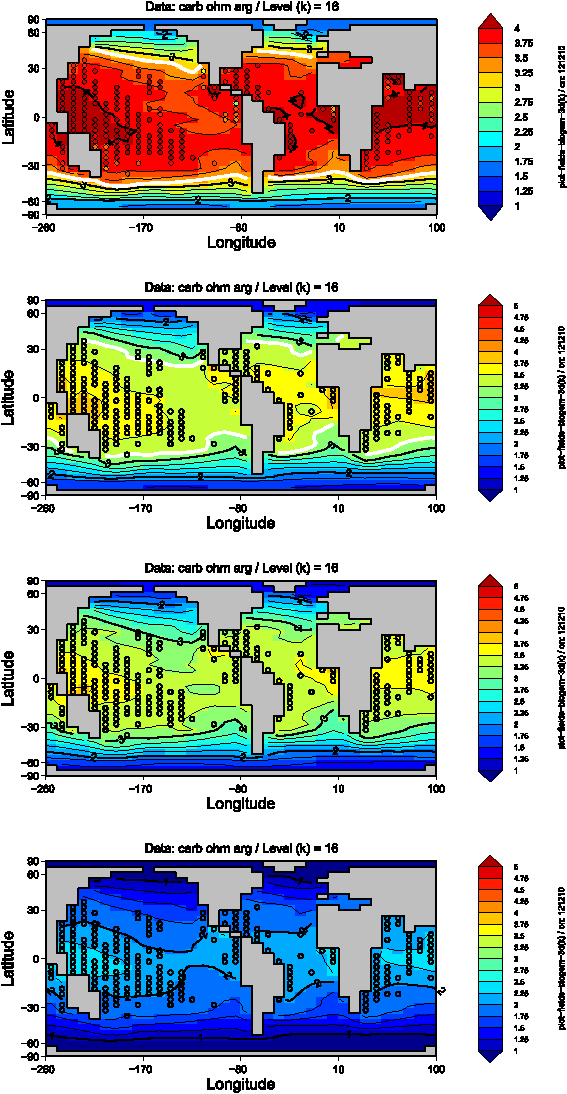
\includegraphics[scale=0.875]{chx-oaimpacts.pdf}
\end{center}
\caption{
\textbf{Mean annual ocean surface saturation (aragonite) changes.}
Top: pre-industrial model ocean surface saturation (aragonite) with ReefBase tropical coral reef locations re-gridded to the \textbf{muffin} grid and color-coded with modern observationally-based saturation values.
2nd and 3rd down: Year 1994 and 2010 ocean surface saturation (aragonite) with ReefBase reef locations.
Bottom: Year 2010 ocean surface saturation (aragonite) under the A2 \(CO_{2}\) emissions scenario.
The thick white line delineates the 3.25 saturation contour (inferred to reflect a limitation on corals).
\textit{Examples here produced using \textbf{muffinplot} but equally do-able in \textbf{Panoply} with the exception of achieving a data overlay. These are provided simply to illustrate some of the impacts you might consider and possible ways of visualizing them.}
}
\label{fig:chx-oaimpacts}
\end{figure}

\begin{figure}[ht]
\begin{center}
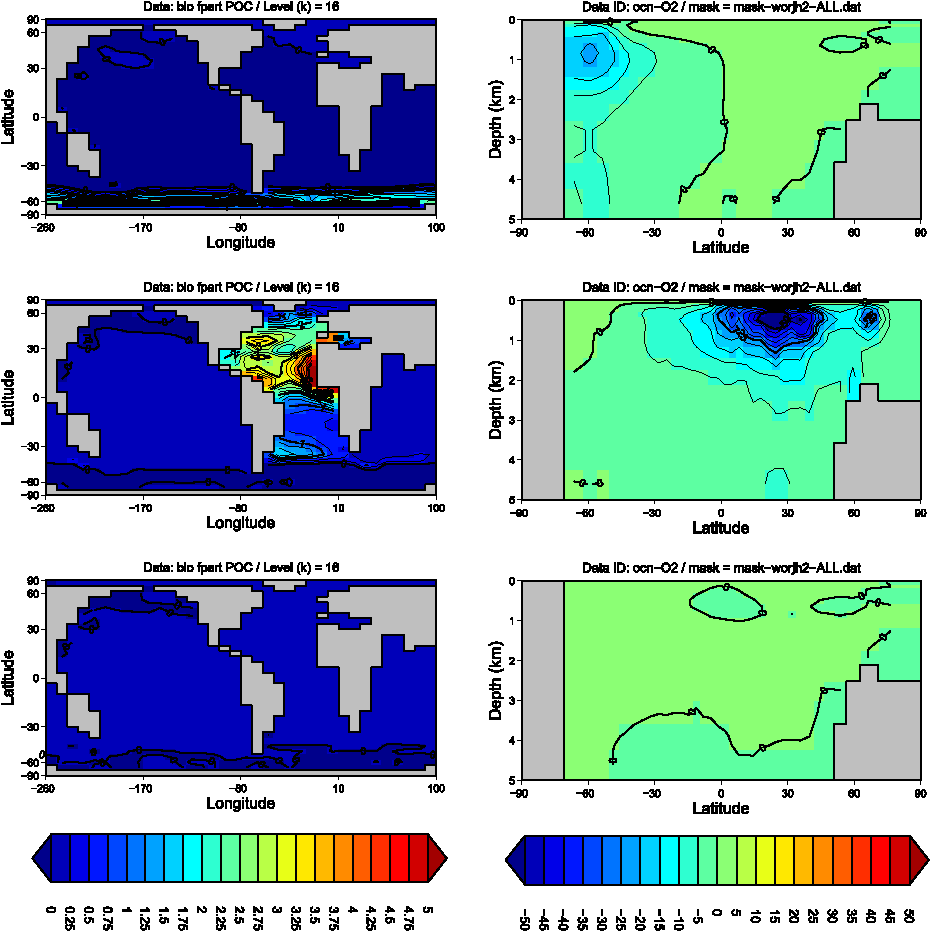
\includegraphics[scale=0.875]{chx-geoengimpacts.pdf}
\end{center}
\caption{
\textbf{Ocean surface export (particulate organic carbon) and zonal \([O_{2}]\) anomalies.}
Left: anomalies of global mean annual export production, for \(Fe\) fertilization (top), \(PO_{4}\) addition (middle), and ocean liming (bottom).
Right: Zonal mean anomalies of dissolved \(O_{2}\) concentrations.
\textit{Examples here produced using \textbf{muffinplot} but equally do-able in \textbf{Panoply} with the exception of achieving a data overlay. These are provided simply to illustrate some of the impacts you might consider and possible ways of visualizing them.}
}
\label{fig:chx-geoengimpacts}
\end{figure}

%------------------------------------------------
\newpage 
%------------------------------------------------

\subsection{Further modifications of the biological pump in the ocean}

Other manipulations of the biological pump and ocean carbon cycle are possible and potentially instructive and in the following examples may be of rather more relevance to past climates and carbon cycles and e.g. possible reasons for the low atmospheric \(CO_{2}\) concentrations at the last glacial, as opposed to relevant to geoengineering (a good thing!). The first two of these may have profound effects not only atmospheric p\(CO_{2}\) but also on dissolved oxygen concentrations in the ocean (and hence implications for the suitability of animal habitat such as for fish) and this is something that you will want to look at as part of your overall assessment of impacts.

%------------------------------------------------

\subsubsection*{Remineralization depth}

\vspace{2mm}
In the model configuration that you have been using, the degradation of particulate organic matter sinking in the water column proceeds according to a fixed profile of flux with depth (there is no e.g. temperature control on the rate of bacterial degradation of sinking organic matter) with \(CO_{2}\) and \(PO_{4}\) released back to the seawater as the particulate flux decreases. The parameter that controls the (\textit{e}-folding) depth scale of particulate organic matter is:
\vspace{-1mm}\small\begin{verbatim}
bg_par_bio_remin_POC_eL1=589.9451
\end{verbatim}\normalsize\vspace{-1mm}
Either edit this value (found under the heading: \texttt{\# --- REMINERALIZATION ---}) or add a new line at the end of the \textit{user-config} file specifying the value you want. Units are \(m\).

\vspace{1mm}
Read \textit{Ridgwell et al.} [2007] for additional discussion of this parameter. See Figure 2-4 in \textit{Ridgwell} [2001] (http://www.seao2.org/pubs/ridgwell\_thesis.pdf) for an illustration of how the flux of particulate organic matter decreases with depth in the ocean, plus references therein.

There is also an associated parameter: \texttt{bg\_par\_bio\_remin\_POC\_frac2}, which sets a fraction of organic matter that is assumed to settle through the water column completely un-altered (currently assigned a value of 0.045 == 4.5\%), but this is arguably less useful to change than the remineralization length-scale of the more labile fraction (the other 95.5\% of particulate organic carbon exported from the ocean surface).

Note that there may well be no simple parallel that can be found in geoengineering to this process. However, there are hypotheses that during the last glacial and as a result of colder ocean temperatures, the depth scale was longer. Conversely, there are ideas about that the warmer temperatures of the e.g. Eocene ocean and hence faster rates of bacterial metabolism led to a much shallower remineralization depth scale. So a remineralization depth scale that is responsive to temperature may have importance in understanding ocean biogeochemical cycles during both past warm and cold climates as well as obviously, future global change. While you are not implementing a temperature-dependent parameterization explicitly, you can at least test for whether changes in temperature might have important impacts by simply changing the remineralization depth to be shallower (smaller depth-scale under a warming climate) or deeper (greater depth-scale in a colder ocean).

%------------------------------------------------

\subsubsection*{Macro nutrient inventory and uptake}

\vspace{2mm}
Suggestions have been made that nutrients were used more efficiently during the LGM, meaning that for the same nutrient uptake at the surface more carbon was exported to depth in the ocean. See: \textit{Omta et al.} [2006]. There are also a bunch of (relatively old) hypotheses concerning differences between glacial and modern ocean in how much nitrate (\(NO^{-}_{3}\)) there was. There is no \(NO^{-}_{3}\) in this version of \textbf{muffin} (just \(PO_{4}\) and \(Fe\)), but an analogous change can be made to the phosphorous cycle.

For the nutrient-to-carbon ratio in organic matter, the relevant parameter is:
\vspace{-1mm}\small\begin{verbatim}
bg_par_bio_red_POP_POC=106.0
\end{verbatim}\normalsize\vspace{-1mm}

\noindent To change the default value (106.0), add a new line at the end of the \textit{user-config} file specifying the value you want. A larger number means that \(PO_{4}\) is being utilized more efficiently and more organic matter is being produced for the same nutrient consumption.

To test the effect of there being more \(PO_{4}\) in the ocean, in addition to using the (surface) flux forcing as described earlier, it is also possible to simply increase the inventory of the ocean as a whole in one go:
\vspace{-1mm}\small\begin{verbatim}
bg_ocn_dinit_8=1.0E-6
\end{verbatim}\normalsize\vspace{-1mm}
which will add \(1\:\mu mol\:kg^{-1}\) of \(PO_{4}\) uniformly to the ocean. (A larger/smaller number will obviously increase the glacial nutrient inventory by more/less.)

In terms of geoengineering, changing the ‘Redfield’ ocean plankton might be difficult … but not impossible, although we are presumably talking about releases of genetically modified organisms to the entire ocean to achieve this meaning there are obviously some severe ethical concerns. However, adding macro nutrients such as \(PO_{4}\) (more often, \(NO^{-}_{3}\) is talked about) may be more feasible.

%------------------------------------------------

\subsubsection*{CaCO3:POC rain ratio}

\vspace{2mm}
Kicked off by a classic 1994 \textit{Nature} paper by \textit{Archer and Maier-Reimer} (see: \textit{Kohfeld and Ridgwell} [2009]), one potential means of changing atmospheric \(CO_{2}\) naturally at the last glacial involves changes in the export ratio between \(CaCO_{3}\) (shells) and \(POC\) (particulate organic matter). Such a change in ratio could come about through a variety of ways (e.g., via the 'silica leakage hypothesis' (see: \textit{Kohfeld and Ridgwell} [2009]) and also through the direct effect of \(Fe\) on diatom physiology (see \textit{Watson et al.} [2000] in \textit{Nature} and also Supplemental Information). There are also ideas about an opposite ocean acidification effect, whereby the less acidic glacial (compared to modern) ocean led to increased calcification and \(CaCO_{3}\) export. Note that this response (higher saturation == greater rate of calcification) is encoded into your model configuration – see \textit{Ridgwell et al.} [2007b].

\vspace{1mm}
In \textbf{muffin}, the \(CaCO_{3}:POC\) rain ratio is controlled (technically: scaled) by the parameter:
\vspace{-1mm}\small\begin{verbatim}
bg_par_bio_red_POC_CaCO3=0.0485
\end{verbatim}\normalsize\vspace{-1mm}

The pattern of \(CaCO_{3}:POC\) rain ratio is not uniform across the ocean (why? (see: \textit{Ridgwell et al.} [2007, 2009]), and its pattern can be viewed in the (2D \textbf{BIOGEM}) netCDF variable: \textsf{\footnotesize misc\_sur\_rCaCO3toPOC}.

(Note that it is unlikely that there is any parallel in a geoengineering context to this process.)

%----------------------------------------------------------------------------------------
%----------------------------------------------------------------------------------------